\subsection{Amélioration de la factorisation et de la résolution triangulaire}
Dans un premier temps, nous allons nous consacrer à l'amélioration de la parallélisation de la factorisation ILU(k).
%
Chaque tâche du graphe de tâches représente la factorisation d'une ligne de la matrice.
%
Cette granularité est trop fine, mais c'est voulu, elle représente la granularité que nous obtenons en décrivant naturellement l'algorithme de la factorisation.
%
Nous avons choisi de simuler deux réservoirs, un cube généré de taille 80 cellules de côté et le réservoir SPE10.
%
Dans le cas du cube, il est possible de choisir le nombre de variables primaires utilisées dans le calcul.
%
Pour rappel, le nombre de variables primaires correspond au nombre de composants simulés.
%
Chaque entrée non-nulle de la matrice correspond à l'interaction entre 2 cellules et sera composée d'une petite matrice dense $Npri*Npri$ avec $Npri$ le nombre de variables primaires.
%
Nous avons choisi de simuler le cube avec 1 variable primaire, 3 variables primaires (modèle {\em black-oil}) et 8 variables primaires (modèle {\em compositionnel}).
%
Pour le réservoir SPE10, c'est un cas {\em black-oil} à 3 variables primaires.
%
Au final nous avons donc 4 matrices différentes.
%
Nous ne faisons pas varier la taille du cube, car les résultats obtenus avec des cubes générés de tailles raisonnablement différentes sont équivalents.

\subsubsection{Sans agrégation}
Nous avons utilisé OpenMP pour tester la parallélisation à grain fin sans agrégation.
%
OpenMP n'ayant pas de gestion de dépendances entre les tâches, nous utiliserons un système de décrémentation atomique.
%
Comme le montrent les résultats de la figure~\ref{fig:res_facto_no_agg}, le nombre de variables primaires a une importance considérable sur les performances que nous obtenons.
%
L'utilisation de 2 threads n'est viable que dans le cas où nous utilisons 8 variables primaires.
%
Dans les autres cas, même en utilisant 4 threads, nous perdons du temps.
%
Ici, le nombre de variables primaires va définir le nombre d'opérations faites par ligne de la matrice, donc plus ce nombre est grand, plus il y aura de travail à faire.
%
Ces résultats confirment notre problème de granularité.
%
Au final, avec l'utilisation des 12 coeurs de calcul de la machine, nous obtenons des accélérations plutôt décevantes, par exemple, pour les cas à 3 variables primaires, le code tourne environ 2,5 fois plus vite que la version séquentielle, mais il utilise 12 fois plus de puissance de calcul.

%   (-_-)   %
\begin{figure}[!h]
  \centering
  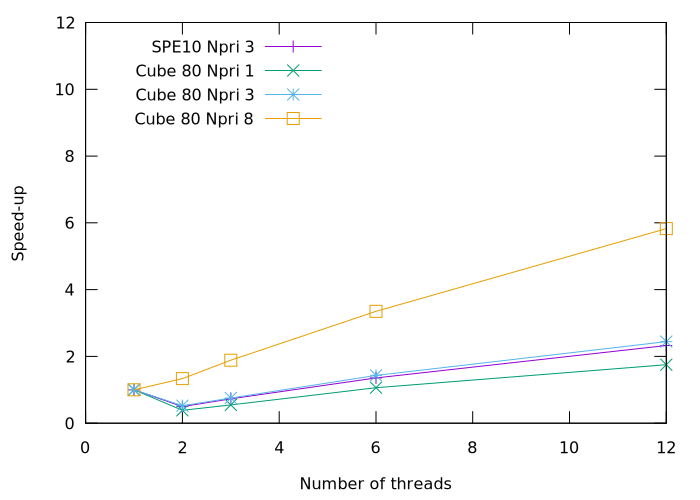
\includegraphics[width=0.7\textwidth]{res_facto_no_agg}
  \caption{Performance de la factorisation sur 12 coeurs sans utiliser Taggre.}
  \label{fig:res_facto_no_agg}
\end{figure}


\subsubsection{Avec l'opérateur F}
Dans un premier temps, nous allons appliquer l'opérateur F avec le paramètre 36.
%
Cet opérateur va donc limiter la largeur du graphe pour qu'il y ait au plus 36 tâches par hauteur du graphe.
%
Nous aurons donc 3 fois plus de tâches que de coeurs de calcul, cela permet de diminuer fortement le nombre de tâches tout en gardant assez de parallélisme pour avoir un bon équilibrage de charge.
%
Nous réduisons donc le parallélisme, mais nous réduisons aussi le nombre de tâches, on divise par 62 le nombre de tâches pour un cube de 80 de côté, nous passons de 512000 tâches à 8232 tâches.
%
Pour le cas SPE10, le nombre de tâches passe de 1094421 à 12896 soit 84 fois moins de tâches.
%
La figure~\ref{fig:res_facto_f36} nous montre une amélioration du temps de factorisation quand le nombre de variables primaires est faible.
%
Cela vient du fait que le surcoût d'ordonnancement de la tâche est du même ordre de grandeur que le temps de calcul de la tâche.
%
Avec 3 variables primaires, la factorisation est 30~\% plus rapide.
%
Avec 1 variable primaire, le temps de factorisation est divisé par 2.
%
Dans le cas où le nombre de variables primaires est élevé, il n'y a pas beaucoup d'amélioration (6~\%).
%
Ici, cet opérateur ne permet pas d'optimiser les accès mémoire caches, seul le surcoût d'ordonnancement est réduit.

%   (-_-)   %
\begin{figure}[!h]
  \centering
  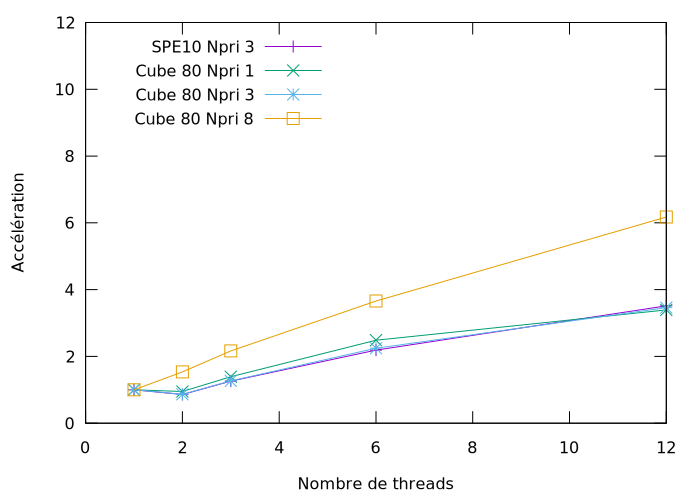
\includegraphics[width=0.7\textwidth]{res_facto_f36}
  \caption{Performance de la factorisation sur 12 coeurs avec Taggre F(36).}
  \label{fig:res_facto_f36}
\end{figure}


\subsubsection{Avec l'opérateur D}
Essayons maintenant l'opérateur D avec le paramètre 8.
%
Cet opérateur va essayer de créer des groupes de 8 tâches assez proches dans le graphe.
%
Nous allons donc diviser par 8 le nombre de tâches, passant ainsi de 512000 tâches à 64000 tâches.
%
Ce qui peut paraître peu mais cette valeur a été choisie empiriquement parmi un ensemble de valeurs.
%
Les autres valeurs donnent des résultats légèrement moins bons, par exemple le paramètre 4 offre une accélération de 3,35, tandis que le paramètre 12 offre 3,55 et finalement le paramètre 8 offre une accélération de 3,72.
%
Comparé à l'opérateur F, il y a très peu d'amélioration quand le nombre de variables primaires est faible (Fig.~\ref{fig:res_facto_d8}).
%
Par contre, avec 8 variables primaires, on obtient un gain de performance qui est dû à une meilleure utilisation des caches, surtout du cache L2 avec une diminution de 10\% des défauts de cache.
%   (-_-)   %
\begin{figure}[!h]
  \centering
  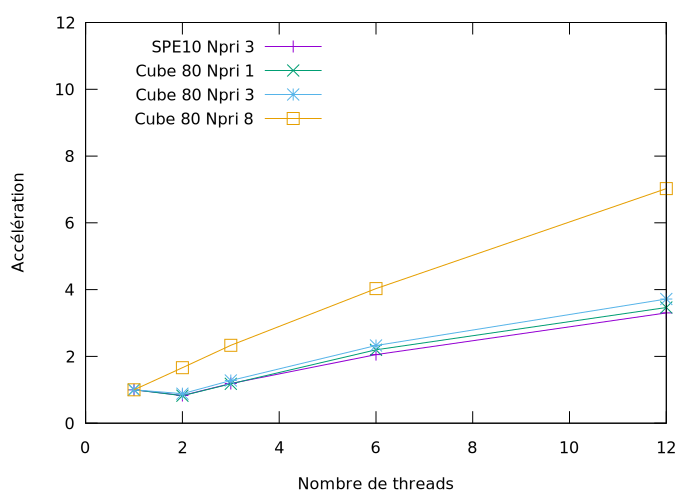
\includegraphics[width=0.7\textwidth]{res_facto_d8}
  \caption{Performance de la factorisation sur 12 coeurs avec Taggre D(8).}
  \label{fig:res_facto_d8}
\end{figure}


\subsubsection{Avec l'opérateur C}
Les deux précédents opérateurs donnent déjà des résultats, mais nous pensons que le meilleur opérateur pour nos matrices reste l'opérateur C.
%
Il a l'avantage de réduire grandement le nombre de tâches comme l'opérateur F et il forme des groupes de tâches permettant une meilleure réusabilité des données en cache.
%
Par contre, il se pourrait que le parallélisme en pâtisse.
%
Comme le montrent les résultats de la figure~\ref{fig:res_facto_c}, tous les cas tests sont améliorés.
%
Il y a bien deux grandes améliorations : la réduction du nombre de tâches et une meilleure réutilisation des caches.
%
Comme pour tous les opérateurs, le nombre de tâches a été réduit, mais dans ce cas la réduction est bien plus importante.
%
Par contre, l'amélioration des effets caches est bien meilleure que dans les autres opérateurs.
%
Cette amélioration est inexistante dans le cas de l'opérateur F, les tâches agrégées n'avaient pas une bonne réutilisabilité des données en cache.
%
Au contraire, l'opérateur D ne réduisait que de très peu le nombre de tâches, mais améliorait la réutilisation des caches.
%
L'opérateur C offre donc le meilleur des deux opérateurs, il produit peu de tâches et en plus ces tâches réutilisent correctement les données en cache.
% L2 stats : F:1.10, D:0.96, C:0.87

%   (-_-)   %
\begin{figure}[!h]
  \centering
  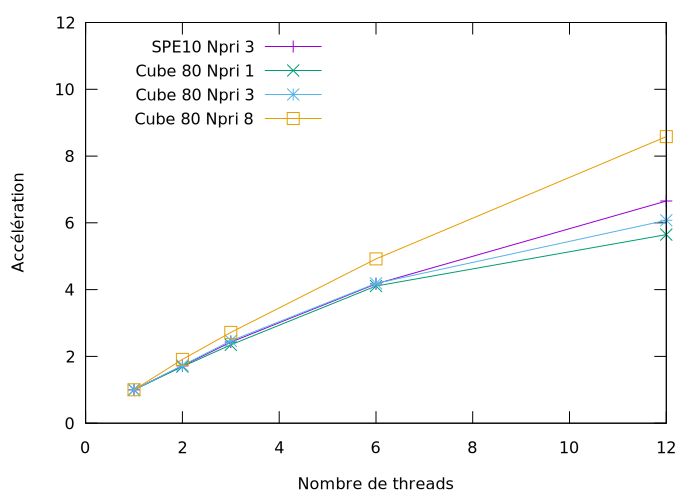
\includegraphics[width=0.7\textwidth]{res_facto_c}
  \caption{Performance de la factorisation sur 12 coeurs avec Taggre C.}
  \label{fig:res_facto_c}
\end{figure}

\subsubsection{Avec plusieurs opérateurs}
Il est aussi possible de combiner plusieurs opérateurs, sur la figure~\ref{fig:res_facto_cd2} nous avons combiné l'opérateur C avec l'opérateur D(2).
%
On observe un très léger gain de performance quand on a une seule variable primaire, mais dans les autres cas on observe le contraire.
%
Malgré ces optimisations, nous n'atteignons pas une accélération parfaite, avec au mieux une accélération de 8,7 pour 12 coeurs.
%
Ce souci de performance est lié à l'architecture mémoire de la machine, nous donnerons plus d'explication dans la partie suivante de la thèse.
%   (-_-)   %
\begin{figure}[!h]
  \centering
  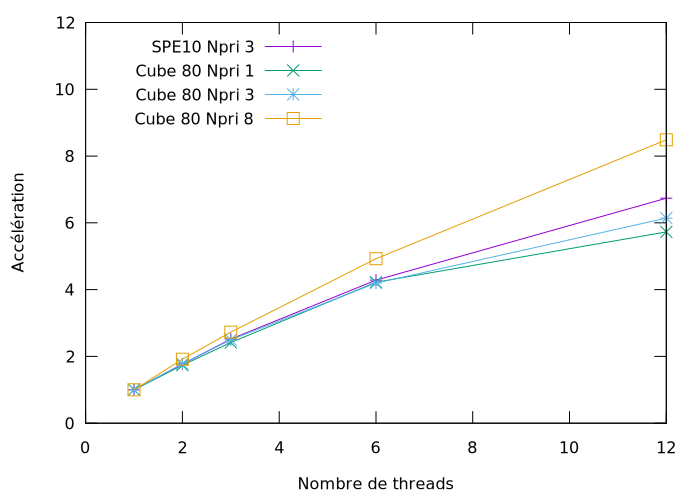
\includegraphics[width=0.7\textwidth]{res_facto_cd2}
  \caption{Performance de la factorisation sur 12 coeurs avec Taggre CD(2).}
  \label{fig:res_facto_cd2}
\end{figure}
\subsubsection{En résumé}

%   (-_-)   %
\begin{center}
  \begin{tabular}{|r|c|c|c|c|c|c|c|c|c|c|}
    \hline
    Type de  &  \multicolumn{5}{c|}{Accélération}  &  \multicolumn{5}{c|}{Nombre de tâches} \\
    matrice  &  \O & F(36) & D(8) & C & CD(2)  &  \O & F(36) & D(8) & C & CD(2)\\
    \hline
    Cube 80 Npri 1 & 1,75 & 3,39 & 3.46 & 5.65 & 5.73 & 512000  & 8232  & 64000  & 6400  & 3200 \\
    Cube 80 Npri 3 & 2,44 & 3,46 & 3.72 & 6.07 & 6.14 & 512000  & 8232  & 64000  & 6400  & 3200 \\
    Cube 80 Npri 8 & 5,83 & 6,17 & 7.02 & 8.58 & 8.48 & 512000  & 8232  & 64000  & 6400  & 3200 \\
    SPE10 Npri 3   & 2,32 & 3,52 & 3.30 & 6.65 & 6.73 & 1094421 & 12896 & 136887 & 36281 & 18181 \\
    \hline
  \end{tabular}
  \captionof{table}{Récapitulatif des résultats de la factorisation sur 12 coeurs de calcul suivant les opérateurs appliqués.}
  \label{tab:facto_res}
\end{center}

\subsubsection{Résultats de la résolution triangulaire}
Essayons maintenant cette technique sur la partie résolution triangulaire du code.
%
Les performances sans agrégation sont bien en dessous de la partie factorisation (Fig.~\ref{fig:res_trsv_no_agg}).
%
Même en utilisant 12 threads, seule la version avec 8 variables primaires donne de meilleurs résultats que la version séquentielle.
%
Encore une fois, il s'agit d'un problème de granularité, le graphe à ordonnancer est le même que pour la factorisation, mais les tâches sont plus petites.

%   (-_-)   %
\begin{figure}[!h]
  \centering
  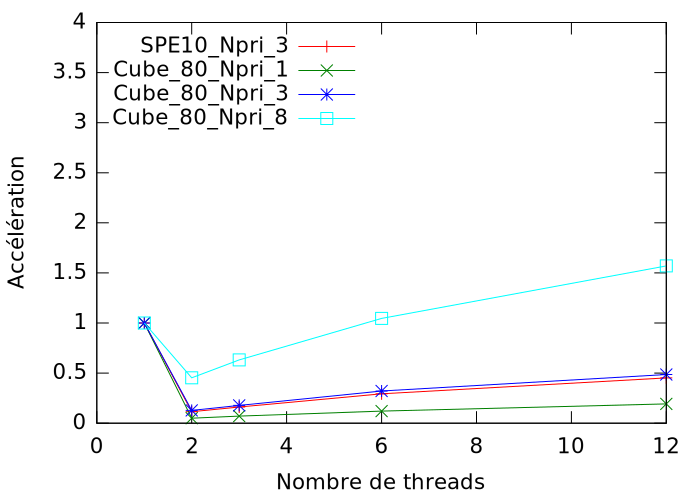
\includegraphics[width=0.7\textwidth]{res_trsv_no_agg}
  \caption{Performance de la résolution triangulaire sur 12 coeurs sans utiliser Taggre.}
  \label{fig:res_trsv_no_agg}
\end{figure}

Si nous regardons les résultats avec la meilleure agrégation que nous ayons, l'agrégation CD(2), on obtient des résultats légèrement meilleurs, mais on n'est encore loin de l'accélération parfaite (Fig.~\ref{fig:res_trsv_cd2}).
%
On arrive ici aux limites de notre méthode, la granularité n'est pas encore suffisante pour permettre d'obtenir de très bonnes performances.
%
Mais si nous augmentons encore la granularité, il n'y aura plus assez de parallélisme pour avoir un bon équilibrage de charge et le temps final sera supérieur.

%   (-_-)   %
\begin{figure}[!h]
  \centering
  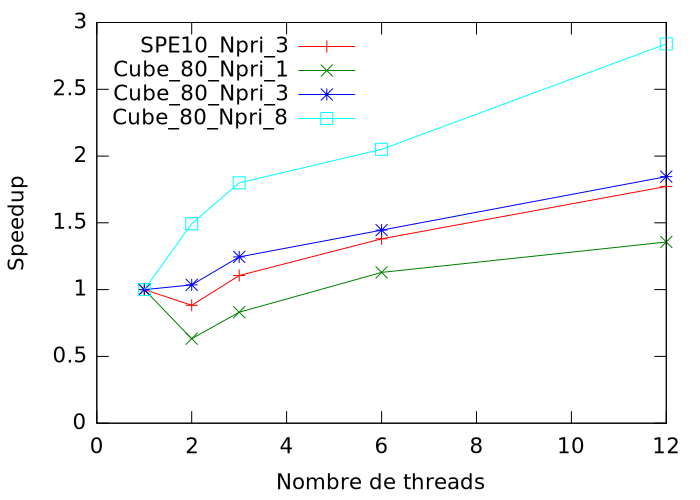
\includegraphics[width=0.7\textwidth]{res_trsv_cd2}
  \caption{Performance de la résolution triangulaire sur 12 coeurs avec Taggre CD(2).}
  \label{fig:res_trsv_cd2}
\end{figure}

%% +---------------------------+-------------+-------------+-------------+------------+
%% |          Metric           |     Sum     |     Max     |     Min     |    Avg     |
%% +---------------------------+-------------+-------------+-------------+------------+
%% | Runtime (RDTSC) [s] STAT  |   1923.94   |   160.328   |   160.328   |  160.328   |
%% | Runtime unhalted [s] STAT |   1870.36   |   160.82    |   152.347   |  155.864   |
%% |     Clock [MHz] STAT      |   34528.4   |   2906.13   |   2850.24   |  2877.37   |
%% |         CPI STAT          |   1.03608   |   1.04174   |   1.02468   | 0.0863398  |
%% |  Data cache misses STAT   | 4.59444e+10 | 4.08753e+09 | 3.71715e+09 | 3.8287e+09 |
%% | Data cache miss rate STAT |   0.10934   | 0.00932521  | 0.00905509  | 0.0091117  |
%% +---------------------------+-------------+-------------+-------------+------------+
%% +---------------------------+-------------+-------------+-------------+-------------+
%% |          Metric           |     Sum     |     Max     |     Min     |     Avg     |
%% +---------------------------+-------------+-------------+-------------+-------------+
%% | Runtime (RDTSC) [s] STAT  |   2004.24   |   167.02    |   167.02    |   167.02    |
%% | Runtime unhalted [s] STAT |   2061.97   |   175.567   |   170.297   |   171.831   |
%% |     Clock [MHz] STAT      |   36151.6   |   3017.39   |   3008.02   |   3012.64   |
%% |         CPI STAT          |   1.14231   |   1.14711   |   1.13205   |  0.0951929  |
%% |  Data cache misses STAT   | 4.87067e+10 | 4.29088e+09 | 4.00937e+09 | 4.05889e+09 |
%% | Data cache miss rate STAT |  0.115926   | 0.00990628  | 0.00962271  | 0.00966052  |
%% +---------------------------+-------------+-------------+-------------+-------------+
%% +---------------------------+-------------+-------------+-------------+-------------+
%% |          Metric           |     Sum     |     Max     |     Min     |     Avg     |
%% +---------------------------+-------------+-------------+-------------+-------------+
%% | Runtime (RDTSC) [s] STAT  |   1640.85   |   136.737   |   136.737   |   136.737   |
%% | Runtime unhalted [s] STAT |   1686.77   |   144.388   |   138.353   |   140.564   |
%% |     Clock [MHz] STAT      |   36255.7   |   3046.34   |   2998.08   |   3021.31   |
%% |         CPI STAT          |  0.934931   |  0.937527   |  0.926718   |  0.0779109  |
%% |  Data cache misses STAT   | 3.85951e+10 | 3.43628e+09 | 3.14135e+09 | 3.21626e+09 |
%% | Data cache miss rate STAT |  0.0919074  | 0.00789712  | 0.00762214  | 0.00765895  |
%% +---------------------------+-------------+-------------+-------------+-------------+


%% +---------------------------+----------+-----------+-----------+-----------+
%% |          Metric           |   Sum    |    Max    |    Min    |    Avg    |
%% +---------------------------+----------+-----------+-----------+-----------+
%% | Runtime (RDTSC) [s] STAT  | 2013.52  |  167.794  |  167.794  |  167.794  |
%% | Runtime unhalted [s] STAT |  2049.5  |  173.386  |  167.781  |  170.792  |
%% |     Clock [MHz] STAT      | 35861.8  |  3005.94  |  2972.33  |  2988.48  |
%% |         CPI STAT          | 1.13698  |  1.14624  |  1.12814  | 0.0947487 |
%% |   L2 request rate STAT    | 0.139712 | 0.0119216 | 0.0115742 | 0.0116426 |
%% |     L2 miss rate STAT     | 0.154052 | 0.0129583 | 0.0127815 | 0.0128376 |
%% |    L2 miss ratio STAT     | 13.2323  |  1.10948  |  1.08696  |  1.10269  |
%% +---------------------------+----------+-----------+-----------+-----------+
%% +---------------------------+----------+-----------+-----------+-----------+
%% |          Metric           |   Sum    |    Max    |    Min    |    Avg    |
%% +---------------------------+----------+-----------+-----------+-----------+
%% | Runtime (RDTSC) [s] STAT  | 1966.96  |  163.913  |  163.913  |  163.913  |
%% | Runtime unhalted [s] STAT | 1886.06  |  158.261  |  156.494  |  157.172  |
%% |     Clock [MHz] STAT      | 34326.8  |  2883.42  |  2837.74  |  2860.57  |
%% |         CPI STAT          | 1.03718  |  1.06006  |  1.01601  | 0.0864318 |
%% |   L2 request rate STAT    | 0.152488 | 0.0130698 | 0.0125945 | 0.0127073 |
%% |     L2 miss rate STAT     | 0.14729  | 0.0125144 | 0.0121436 | 0.0122742 |
%% |    L2 miss ratio STAT     | 11.5912  | 0.970545  | 0.957504  | 0.965933  |
%% +---------------------------+----------+-----------+-----------+-----------+
%% +---------------------------+----------+-----------+-----------+-----------+
%% |          Metric           |   Sum    |    Max    |    Min    |    Avg    |
%% +---------------------------+----------+-----------+-----------+-----------+
%% | Runtime (RDTSC) [s] STAT  |  1652.6  |  137.716  |  137.716  |  137.716  |
%% | Runtime unhalted [s] STAT | 1694.79  |  142.824  |  140.196  |  141.233  |
%% |     Clock [MHz] STAT      | 36166.7  |  3035.99  |  2993.16  |  3013.9   |
%% |         CPI STAT          | 0.937105 | 0.962554  | 0.921956  | 0.0780921 |
%% |   L2 request rate STAT    | 0.158081 | 0.0134666 | 0.0131121 | 0.0131734 |
%% |     L2 miss rate STAT     | 0.138087 | 0.0116948 | 0.0114514 | 0.0115072 |
%% |    L2 miss ratio STAT     | 10.4823  |  0.87775  |  0.86843  | 0.873526  |
%% +---------------------------+----------+-----------+-----------+-----------+

%% +---------------------------+----------+-----------+---------+------------+
%% |          Metric           |   Sum    |    Max    |   Min   |    Avg     |
%% +---------------------------+----------+-----------+---------+------------+
%% | Runtime (RDTSC) [s] STAT  | 2014.07  |  167.839  | 167.839 |  167.839   |
%% | Runtime unhalted [s] STAT | 2045.66  |  172.625  | 168.205 |  170.471   |
%% |     Clock [MHz] STAT      | 35826.2  |  3000.16  | 2971.72 |  2985.52   |
%% |         CPI STAT          | 1.13743  |  1.14473  | 1.12957 | 0.0947856  |
%% |   L3 request rate STAT    | 0.085237 | 0.0429422 |    0    | 0.00710308 |
%% |     L3 miss rate STAT     | 0.116483 | 0.0586274 |    0    | 0.00970692 |
%% |    L3 miss ratio STAT     |  1.1549  | 0.577687  |    0    | 0.0962418  |
%% +---------------------------+----------+-----------+---------+------------+
%% +---------------------------+-----------+-----------+---------+------------+
%% |          Metric           |    Sum    |    Max    |   Min   |    Avg     |
%% +---------------------------+-----------+-----------+---------+------------+
%% | Runtime (RDTSC) [s] STAT  |  1932.6   |  161.05   | 161.05  |   161.05   |
%% | Runtime unhalted [s] STAT |  1869.75  |  159.171  | 152.621 |  155.813   |
%% |     Clock [MHz] STAT      |  34423.7  |  2896.06  | 2841.43 |  2868.64   |
%% |         CPI STAT          |  1.03599  |  1.03868  | 1.03237 | 0.0863323  |
%% |   L3 request rate STAT    | 0.0858767 | 0.0432998 |    0    | 0.00715639 |
%% |     L3 miss rate STAT     | 0.106569  | 0.0534681 |    0    | 0.00888075 |
%% |    L3 miss ratio STAT     |  1.10754  | 0.554997  |    0    | 0.0922947  |
%% +---------------------------+-----------+-----------+---------+------------+
%% +---------------------------+-----------+-----------+----------+------------+
%% |          Metric           |    Sum    |    Max    |   Min    |    Avg     |
%% +---------------------------+-----------+-----------+----------+------------+
%% | Runtime (RDTSC) [s] STAT  |  1696.46  |  141.372  | 141.372  |  141.372   |
%% | Runtime unhalted [s] STAT |  1699.84  |  146.474  | 137.316  |  141.654   |
%% |     Clock [MHz] STAT      |  35865.4  |  3011.87  | 2965.87  |  2988.79   |
%% |         CPI STAT          | 0.931982  | 0.946119  | 0.924821 | 0.0776651  |
%% |   L3 request rate STAT    | 0.0785352 | 0.0400494 |    0     | 0.0065446  |
%% |     L3 miss rate STAT     | 0.0962549 | 0.0481313 |    0     | 0.00802125 |
%% |    L3 miss ratio STAT     |  1.10147  |  0.55564  |    0     | 0.0917888  |
%% +---------------------------+-----------+-----------+----------+------------+

%% +---------------------------------+------------+-------------+-------------+-------------+
%% |             Metric              |    Sum     |     Max     |     Min     |     Avg     |
%% +---------------------------------+------------+-------------+-------------+-------------+
%% |    Runtime (RDTSC) [s] STAT     |  2070.55   |   172.546   |   172.546   |   172.546   |
%% |    Runtime unhalted [s] STAT    |  2068.93   |   175.779   |   169.669   |   172.411   |
%% |        Clock [MHz] STAT         |  35538.6   |   3007.39   |   2915.92   |   2961.55   |
%% |            CPI STAT             |  1.13513   |   1.15526   |   1.11284   |  0.094594   |
%% |        Branch rate STAT         |  0.905246  |  0.0790124  |  0.0746446  |  0.0754372  |
%% | Branch misprediction rate STAT  | 0.00516248 | 0.000476814 | 0.000405921 | 0.000430207 |
%% | Branch misprediction ratio STAT | 0.0684119  | 0.00618842  | 0.00543805  | 0.00570099  |
%% |  Instructions per branch STAT   |  159.109   |   13.3968   |   12.6562   |   13.2591   |
%% +---------------------------------+------------+-------------+-------------+-------------+
%% +---------------------------------+------------+-------------+-------------+-------------+
%% |             Metric              |    Sum     |     Max     |     Min     |     Avg     |
%% +---------------------------------+------------+-------------+-------------+-------------+
%% |    Runtime (RDTSC) [s] STAT     |  1961.67   |   163.472   |   163.472   |   163.472   |
%% |    Runtime unhalted [s] STAT    |  1876.49   |   158.39    |   154.522   |   156.374   |
%% |        Clock [MHz] STAT         |  34367.1   |   2882.84   |   2844.95   |   2863.92   |
%% |            CPI STAT             |   1.0338   |   1.05326   |   1.01697   |  0.0861503  |
%% |        Branch rate STAT         |  0.897154  |  0.0761396  |  0.0736554  |  0.0747628  |
%% | Branch misprediction rate STAT  | 0.00511161 | 0.000463287 | 0.000395029 | 0.000425968 |
%% | Branch misprediction ratio STAT | 0.0683374  | 0.00613752  | 0.00536154  | 0.00569478  |
%% |  Instructions per branch STAT   |  160.529   |   13.5767   |   13.1338   |   13.3774   |
%% +---------------------------------+------------+-------------+-------------+-------------+



%% +---------------------------+---------+---------+---------+-----------+
%% |          Metric           |   Sum   |   Max   |   Min   |    Avg    |
%% +---------------------------+---------+---------+---------+-----------+
%% | Runtime (RDTSC) [s] STAT  | 1961.79 | 163.482 | 163.482 |  163.482  |
%% | Runtime unhalted [s] STAT | 1874.13 | 160.463 | 152.47  |  156.177  |
%% |     Clock [MHz] STAT      | 34317.2 | 2879.83 | 2839.8  |  2859.77  |
%% |         CPI STAT          | 1.0348  | 1.05031 | 1.02074 | 0.0862334 |
%% | Load to Store ratio STAT  | 44.4467 | 3.72245 | 3.6765  |  3.70389  |
%% +---------------------------+---------+---------+---------+-----------+
